The experiments can be split up into three different parts inspecting how ToMe affects performance\\ \(1)\) when applied to different parts of the transformer,\\ \(2)\) when applied to smaller images, and\\ \(3)\) when different settings for partitioning the \textbf{src} and \textbf{dst} sets are used.\\
\\
The results of every experimental unit are presented in two figures. The first figure focuses on image quality, displaying FID values, while the subsequent one emphasizes image generation speed by showcasing how the average time required for image generation of each subset compares to the \(r=0\%\) subset.
Both figures have \(r\%\) on the x-axis showing how the metrics change with an increasing amount of tokens merged.\\
Datasets that are compared in an experimental unit, were always created with the same set of prompts and seeds, to ensure the comparability of the results.



\subsubsection*{1): Experimenting with different components of the transformer}
ToMe's default configuration involves token merging solely within the self-attention module.
Our first set of experiments aims to gauge how the performance metrics are affected when creating sets of $768 \times 768$ images, by extending token merging to different combinations of transformer components.



\subsubsection*{1.1): default (only self-attn) vs all (self-attn, cross-attn and mlp)}
The first experiment of part 1 compares the default setting of ToMe where token merging is only applied in the self-attn layer (black) with a different configuration that has token merging applied in the self-attn, cross-attn and mlp layer (red). 
\begin{figure}[!htb]
\label{fig:exp_1_1}
   % FID values for run2 and run3
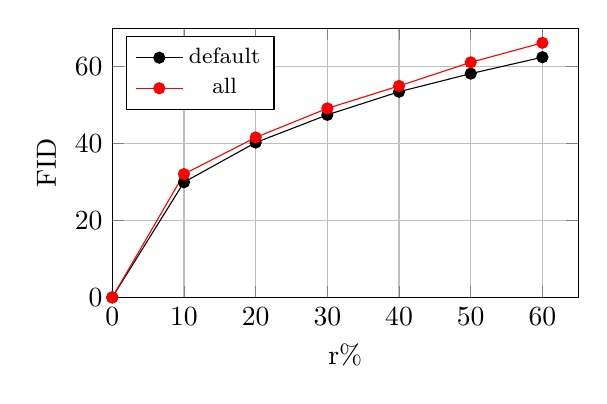
\begin{tikzpicture}
\begin{axis}[
    title={},
    height=5cm,
    width=7.5cm,
    xlabel={r\%},
    ylabel={FID},
    xmin=0, xmax=65,
    ymin=0, ymax=70,
    xtick={0,10,20,30,40,50,60},
    ytick={0,20,40,60},
    legend pos=north west,
    xmajorgrids=true,
    ymajorgrids=true,
    legend style={font=\footnotesize}
]

\addplot[
    color=black,
    mark=*
    ]
    coordinates {
    (0,0)(10,29.95)(20,40.26)(30,47.47)(40,53.48)(50,58.19)(60,62.46)
    };
    
\addplot[
    color=red,
    mark=*
    ]
    coordinates {
    (0,0)(10,32.07)(20,41.60)(30,49.15)(40,54.99)(50,61.13)(60,66.20)
    };
    
\legend{default, all}
    
\end{axis}
\end{tikzpicture}
   % time values for run2 and run3
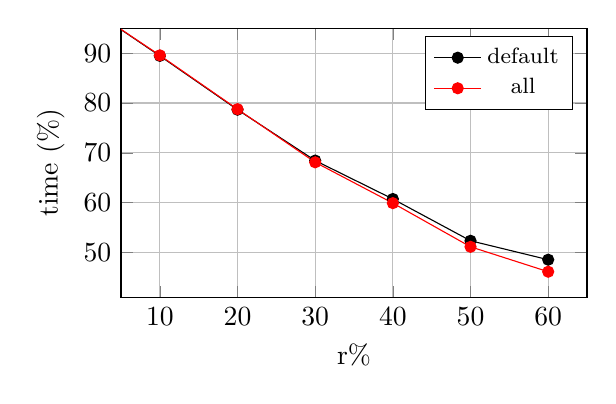
\begin{tikzpicture}
\begin{axis}[
    title={},
    height=5cm,
    width=7.5cm,
    xlabel={r\%},
    ylabel={time (\%)},
    xmin=5, xmax=65,
    ymin=41, ymax=95,
    xtick={10,20,30,40,50,60},
    ytick={50,60,70,80,90},
    legend pos=north east,
    xmajorgrids=true,
    ymajorgrids=true,
    legend style={font=\footnotesize}
]

\addplot[
    color=black,
    mark=*
    ]
    coordinates {
    (0,100)(10,89.45)(20,78.65)(30,68.45)(40,60.74)(50,52.36)(60,48.56)
    };
    
\addplot[
    color=red,
    mark=*
    ]
    coordinates {
    (0,100)(10,89.56)(20,78.76)(30,68.10)(40,59.91)(50,51.15)(60,46.15)
    };
    
\legend{default, all}
    
\end{axis}
\end{tikzpicture}
\caption{FID and relative time compared to r=0\% for 1.1)}
\label{fig:exp_1_1}
\end{figure}\\
%\newpage
Firstly, the default setup of ToMe does make inference up to \(2 \times\) faster for \(r = 50\%\) (see Tab.~\ref{table:exp_1_1}), matching Bolya and Hoffman's description.\\
The naive approach to improve performance by using token merging in every transformer layer, seemingly does not yield significant improvements as image generation speed noticeably increases when \(r > 30\%\), albeit at a clear cost of image quality with FID being consistently larger for this configuration (see Fig.~\ref{fig:exp_1_1}). \\
ToMe, in its default setup, consistently produces images closer to their no-ToMe original, so extending token merging to both the cross-attn and mlp layer does not appear beneficial. This approach can therefore be disregarded.



%\newpage
\subsubsection*{1.2): [default] vs [self-attn \& cross-attn] vs [self-attn \& mlp]}
After \(1.1\), the question remains whether performance drops were caused by using ToMe in both the cross-attn and mlp layer or only one of them, so the second experiment of part 1 attempts to delve deeper into that matter. This time token merging is only extended to either the cross-attn (red) or the mlp module (blue). Then a comparison is made with the results of the default ToMe settings (black) from the previous trial.
\begin{figure}[!htb]
    % FID values for run2, run4 and run5
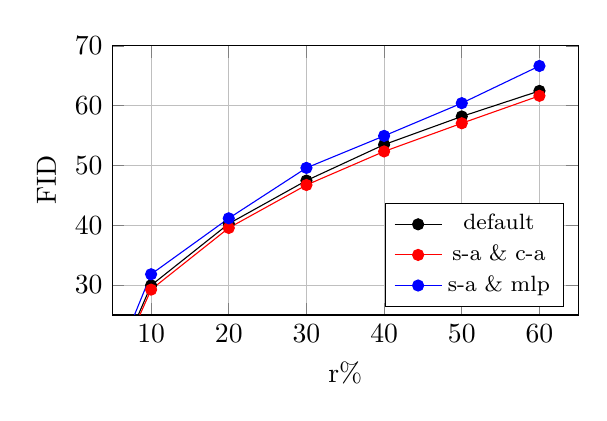
\begin{tikzpicture}
\begin{axis}[
    title={},
    height=5cm,
    width=7.5cm,
    xlabel={r\%},
    ylabel={FID},
    xmin=5, xmax=65,
    ymin=25, ymax=70,
    xtick={10,20,30,40,50,60},
    ytick={30,40,50,60,70},
    legend pos=south east,
    xmajorgrids=true,
    ymajorgrids=true,
    legend style={font=\footnotesize}
]

\addplot[
    color=black,
    mark=*
    ]
    coordinates {
    (0,0)(10,29.95)(20,40.26)(30,47.47)(40,53.48)(50,58.19)(60,62.46)
    };
    
\addplot[
    color=red,
    mark=*
    ]
    coordinates {
    (0,0)(10,29.24)(20,39.55)(30,46.73)(40,52.34)(50,57.05)(60,61.64)
    };

\addplot[
    color=blue,
    mark=*
    ]
    coordinates {
    (0,0)(10,31.81)(20,41.16)(30,49.59)(40,54.94)(50,60.41)(60,66.63)
    };
    
\legend{default, s-a \& c-a, s-a \& mlp}
    
\end{axis}
\end{tikzpicture}
    % time values for run2, run4 and run5
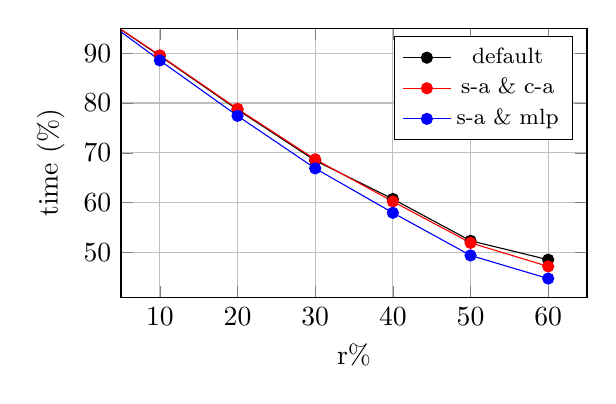
\begin{tikzpicture}
\begin{axis}[
    title={},
    height=5cm,
    width=7.5cm,
    xlabel={r\%},
    ylabel={time (\%)},
    xmin=5, xmax=65,
    ymin=41, ymax=95,
    xtick={10,20,30,40,50,60},
    ytick={50,60,70,80,90},
    legend pos=north east,
    xmajorgrids=true,
    ymajorgrids=true,
    legend style={font=\footnotesize}
]
    
\addplot[
    color=black,
    mark=*
    ]
    coordinates {
    (0,100)(10,89.45)(20,78.65)(30,68.45)(40,60.74)(50,52.36)(60,48.56)
    };

\addplot[
    color=red,
    mark=*
    ]
    coordinates {
    (0,100)(10,89.55)(20,78.82)(30,68.70)(40,60.24)(50,51.94)(60,47.21)
    };

\addplot[
    color=blue,
    mark=*
    ]
    coordinates {
    (0,100)(10,88.54)(20,77.42)(30,66.88)(40,57.97)(50,49.42)(60,44.78)
    };

    
\legend{default, s-a \& c-a, s-a \& mlp}
    
\end{axis}
\end{tikzpicture}
\caption{FID and relative time compared to r=0\% for 1.2)}
\label{fig:exp_1_2}
\end{figure}\\
%\newpage
This time it's clearly visible that merging tokens within the self-attn and cross-attn module performs the best, as it slightly improves the ToMe defualt both in terms of image quality and image generation speed when \(r > 30\%\) (see Fig.~\ref{fig:exp_1_2}).\\
Token merging in the self-attn and mlp module on the other hand might offer the biggest speedup for image generation, but clearly performs the worst in terms of image quality across the board (see Tab.~\ref{table:exp_1_2}).\\
We can therefore conclude that extending token merging to the cross-attn module might have positive effects on the performance, while extending it to the mlp module clearly worsens image quality.



%\newpage
\subsubsection*{1.3): [default] vs [cross-attn \& mlp] vs [only cross-attn]}
The common denominator of the previous examinations was the application of token merging in the self-attn layer. This time we are explicitly avoiding token merging in the self-attn module and instead apply it in only the cross-attn (blue) and both the cross-attn and mlp component (red).
The results of the default ToMe settings (black) again carry over from the previous trial.\\
\begin{figure}[!htb]
    % FID values for run10 and run11
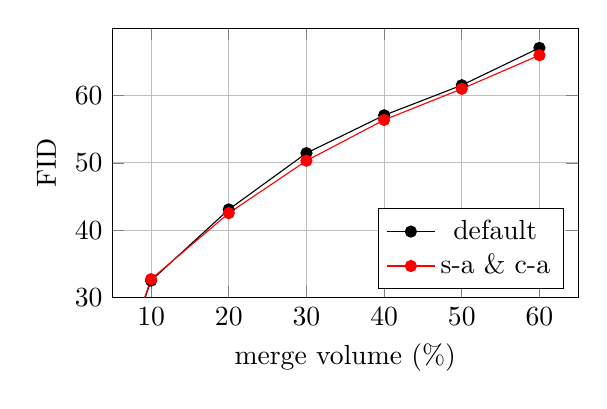
\begin{tikzpicture}
\begin{axis}[
    title={},
    height=5cm,
    width=7.5cm,
    xlabel={merge volume (\%)},
    ylabel={FID},
    xmin=5, xmax=65,
    ymin=30, ymax=70,
    xtick={10,20,30,40,50,60},
    ytick={30,40,50,60},
    legend pos=south east,
    xmajorgrids=true,
    ymajorgrids=true,
]

\addplot[
    color=black,
    mark=*
    ]
    coordinates {
    (0,0)(10,32.49)(20,43.07)(30,51.44)(40,57.06)(50,61.53)(60,67.08)
    };
    
\addplot[
    color=red,
    mark=*
    ]
    coordinates {
    (0,0)(10,32.71)(20,42.52)(30,50.31)(40,56.37)(50,60.99)(60,65.99)
    };
    
\legend{default, s-a \& c-a}
    
\end{axis}
\end{tikzpicture}
    % time values for run10 and run11
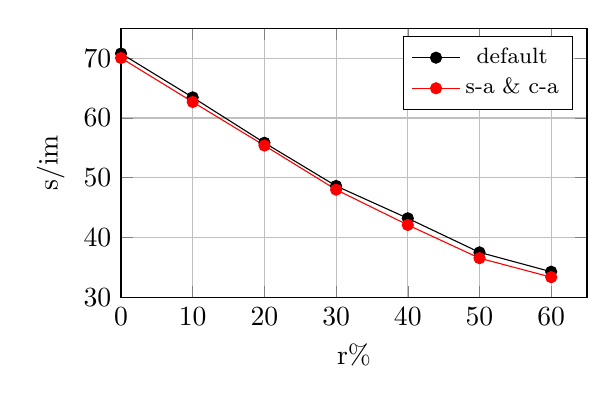
\begin{tikzpicture}
\begin{axis}[
    title={},
    height=5cm,
    width=7.5cm,
    xlabel={r\%},
    ylabel={s/im},
    xmin=0, xmax=65,
    ymin=30, ymax=75,
    xtick={0,10,20,30,40,50,60},
    ytick={30,40,50,60,70},
    legend pos=north east,
    xmajorgrids=true,
    ymajorgrids=true,
    legend style={font=\footnotesize}
]

\addplot[
    color=black,
    mark=*
    ]
    coordinates {
    (0,70.77)(10,63.44)(20,55.85)(30,48.63)(40,43.22)(50,37.53)(60,34.29)
    };
    
\addplot[
    color=red,
    mark=*
    ]
    coordinates {
    (0,70.02)(10,62.67)(20,55.39)(30,48.01)(40,42.11)(50,36.56)(60,33.38)
    };
    
\legend{default, s-a \& c-a}
    
\end{axis}
\end{tikzpicture}
\caption{FID and relative time compared to r=0\% for 1.3)}
\label{fig:exp_1_3}
\end{figure}\\
The most striking result here is that no token merging in the self-attn layer corresponds to no image generation speedup at all, rather slowing the process down (see Tab.~\ref{table:exp_1_3}). 
The apparent improvements to image quality compared to the ToMe default (see Fig.~\ref{fig:exp_1_3}) consequently become negligible without any speed benefits, though it can be noted that token merging in only the cross-attn layer greatly outperforms token merging in both cross-attn and mlp layer in terms of image quality.\\
We conclusively derive that ToMe without involvement of the self-attn layer does not accelerate the image generation process at all and can be considered redundant and therefore be disregarded. It can additionally be derived from \(1.1 - 1.3\) that token merging in the mlp layer has strong negative effects on image quality and, thus, can not be recommended.




%\newpage
\subsubsection*{1.4): [default] vs [self-attn \& cross-attn] (the second time)}
The most prominent takeaway of the first three experiments is that token merging in both the self-attn and cross-attn layers improves the performance of ToMe both in terms of image quality and image generation speed.\\
We want to further examine this discovery by repeating the experiment with a new set of 500 different prompt-seed pairs and then average the results of both trials.
\begin{figure}[!htb]
    % FID values for run10 and run11
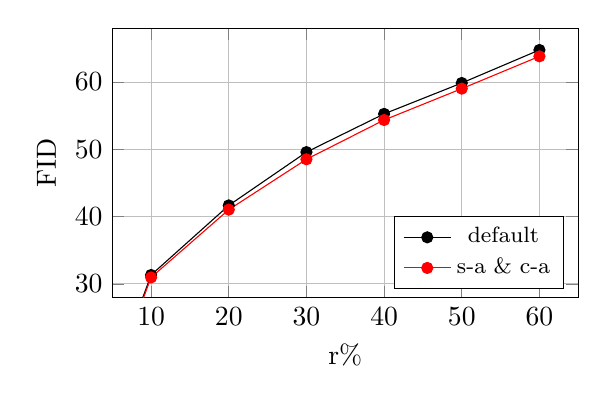
\begin{tikzpicture}
\begin{axis}[
    title={},
    height=5cm,
    width=7.5cm,
    xlabel={r\%},
    ylabel={FID},
    xmin=5, xmax=65,
    ymin=28, ymax=68,
    xtick={10,20,30,40,50,60},
    ytick={30,40,50,60},
    legend pos=south east,
    xmajorgrids=true,
    ymajorgrids=true,
    legend style={font=\footnotesize}
]

\addplot[
    color=black,
    mark=*
    ]
    coordinates {
    (0,0)(10,31.33)(20,41.67)(30,49.59)(40,55.27)(50,59.86)(60,64.77)
    };
    
\addplot[
    color=red,
    mark=*
    ]
    coordinates {
    (0,0)(10,30.97)(20,41.04)(30,48.52)(40,54.36)(50,59.02)(60,63.82)
    };
    
\legend{default, s-a \& c-a}
    
\end{axis}
\end{tikzpicture}
    % time values for run10 and run11
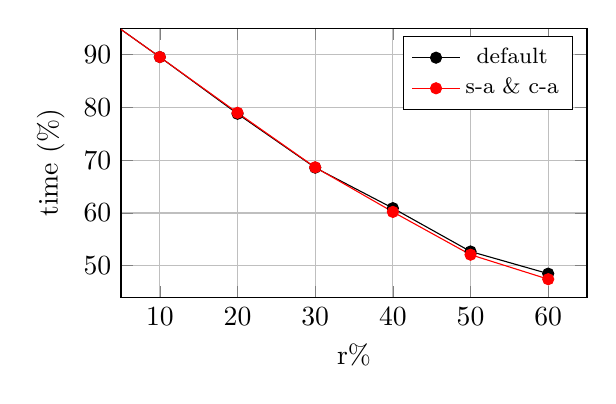
\begin{tikzpicture}
\begin{axis}[
    title={},
    height=5cm,
    width=7.5cm,
    xlabel={r\%},
    ylabel={time (\%)},
    xmin=5, xmax=65,
    ymin=44, ymax=95,
    xtick={10,20,30,40,50,60},
    ytick={50,60,70,80,90},
    legend pos=north east,
    xmajorgrids=true,
    ymajorgrids=true,
    legend style={font=\footnotesize}
]

\addplot[
    color=black,
    mark=*
    ]
    coordinates {
    (0,100)(10,89.54)(20,78.79)(30,68.58)(40,60.91)(50,52.70)(60,48.50)
    };
    
\addplot[
    color=red,
    mark=*
    ]
    coordinates {
    (0,100)(10,89.54)(20,78.98)(30,68.65)(40,60.20)(50,52.09)(60,47.45)
    };
    
\legend{default, s-a \& c-a}
    
\end{axis}
\end{tikzpicture}
\caption{FID and relative time compared to r=0\% for 1.4)}
\label{fig:exp_1_4}
\end{figure}\\
%\newpage
It is again visible that the use of ToMe in both the self-attn and cross-attn layer, firstly, improves image quality in any case and improves inference speed when \(r > 30\%\) compared to the ToMe default (see Fig.~\ref{fig:exp_1_4}). Image generation speed seems unaffected by ToMe when \(r \leq 30\%\) (see Tab.~\ref{table:exp_1_4}).
These results motivate the use of token merging in both the self-attn and cross-attn modules as the new default for $768 \times 768$ images going forward.



%\newpage
\subsubsection*{2): Exploring smaller images sizes}
In this section, we want to expand the scope of our trials to smaller image sizes. Precisely, we want to repeat looking at token merging in the self-attn layer (black) and both the self-attn and cross-attn layer (red), but this time with smaller $512 \times 512$ images. Again a set of 500 prompts is randomly sampled and a corresponding set of random seeds is generated.
\begin{figure}[!htb]
    % FID values for run8 and run9
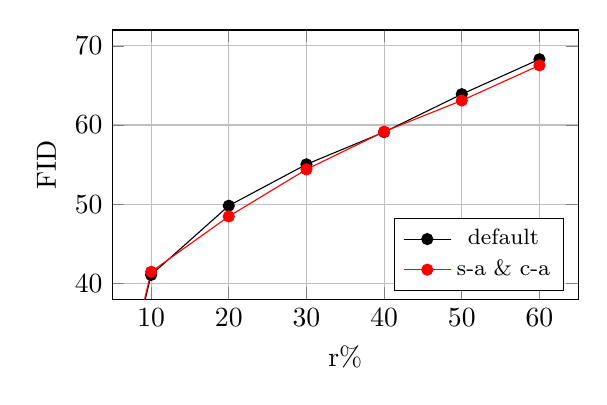
\begin{tikzpicture}
\begin{axis}[
    title={},
    height=5cm,
    width=7.5cm,
    xlabel={r\%},
    ylabel={FID},
    xmin=5, xmax=65,
    ymin=38, ymax=72,
    xtick={10,20,30,40,50,60},
    ytick={30,40,50,60,70},
    legend pos=south east,
    xmajorgrids=true,
    ymajorgrids=true,
    legend style={font=\footnotesize}
]

\addplot[
    color=black,
    mark=*
    ]
    coordinates {
    (0,0)(10,41.06)(20,49.80)(30,55.03)(40,59.10)(50,63.89)(60,68.30)
    };
    
\addplot[
    color=red,
    mark=*
    ]
    coordinates {
    (0,0)(10,41.45)(20,48.45)(30,54.39)(40,59.16)(50,63.09)(60,67.53)
    };
    
\legend{default, s-a \& c-a}
    
\end{axis}
\end{tikzpicture}
    % time values for run2, run6 and run7
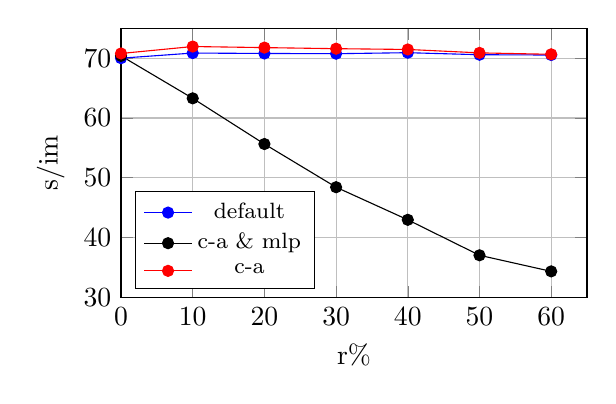
\begin{tikzpicture}
\begin{axis}[
    title={},
    height=5cm,
    width=7.5cm,
    xlabel={r\%},
    ylabel={s/im},
    xmin=0, xmax=65,
    ymin=30, ymax=75,
    xtick={0,10,20,30,40,50,60},
    ytick={30,40,50,60,70},
    legend pos=south west,
    xmajorgrids=true,
    ymajorgrids=true,
    legend style={font=\footnotesize}
]

\addplot[
    color=blue,
    mark=*
    ]
    coordinates {
    (0,69.99)(10,70.85)(20,70.78)(30,70.74)(40,70.91)(50,70.57)(60,70.52)
    };

\addplot[
    color=black,
    mark=*
    ]
    coordinates {
    (0,70.38)(10,63.28)(20,55.64)(30,48.42)(40,42.97)(50,37.04)(60,34.35)
    };
    
\addplot[
    color=red,
    mark=*
    ]
    coordinates {
    (0,70.78)(10,71.94)(20,71.76)(30,71.58)(40,71.45)(50,70.88)(60,70.64)
    };

    
\legend{default, c-a \& mlp, c-a}
    
\end{axis}
\end{tikzpicture}
\caption{FID and relative time compared to r=0\% for 2)}
\label{fig:exp_2}
\end{figure}\\
%\newpage
Generally, the speedup provided by ToMe noticeably decreases to ~25\% from ~50\% in the previous trials with \(768 \times 768\) images. ToMe even worsens image generation speed when \(r<20\%\), as the image generation process actually becomes slower by about 1 s/im at \(r=10\%\) (see Tab.~\ref{table:exp_2}).\\
The inclusion of the cross-attn layer provides a consistent time improvement, but image quality gains are quite inconsistent.
ToMe in self- and cross-attn yields better quality for \(r>10\%\) but the gap closes completely at \(r=40\%\) (see Fig.~\ref{fig:exp_2}).\\
We conclude that using ToMe for such small images (e.g. $512 \times 512$ or smaller) is less practical than it is for larger images. It is especially inadvisable to be used with a small merge volume \((r<20\%)\), as there is no time gained in the diffusion process, but information is lost during merging. \\
In consequence, we will not investigate the usage of ToMe on this scale any further. Neither will we investigate ToMe's effect on larger images due to hardware limitations.



%\newpage
\subsubsection*{3): Exploring different batch sizes}
The third part of the experimental section examines, how different values for \(sx\) and \(sy\) influence the performance of ToMe on $768 \times 768$ images. As a reminder, \(sx\) and \(sy\) determine the size of the token batches, which are used to spread the \textbf{dst} tokens somewhat evenly across the image, with larger batches resulting in a less consistent distribution. Our new default of ToMe with token merging applied in both the self-attn and cross-attn layer will be used throughout this section.



%\newpage
\subsubsection*{3.1): $3 \times 3$ batches}
The first choice was scaling up from $2 \times 2$ (black) to $3 \times 3$ batches (red). This setup strongly tilts the ratio of src and dst tokens toward the former and theoretically allows for a larger number of tokens to be merged. 
\begin{align*}
    r_{max} = 1-\frac{1}{3*3} = \frac{8}{9} \approx 88.89\%
\end{align*}
We will, nevertheless, not exceed a merge rate of \(r=60\%\), as image quality already exhibits clear deterioration at that level and also due to the absence of other data available for comparison.



\subsubsection*{3.2): $1 \times 2$ vertical batches}
Scaling down the same way to $1 \times 1$ batches is impossible, as it would result in every token landing in the \textbf{dst} set and \(r_{max}=0\%\).\\
We therefore chose to cut the batches in half horizontally, creating $1 \times 2$ batches. This decision led to a balanced 50-50 distribution between \textbf{src} and \textbf{dst}.
\begin{align*}
    r_{max} = 1-\frac{1}{1*2} = 50\%
\end{align*}
This limits our merge volume to 50\% but allows for better matches during the merge process. Compared to the $2 \times 2$ default, every \textbf{src} token now has double the number of \textbf{dst} tokens to be matched with.\\
\begin{figure}[!htb]
    % FID values for run11, run14 and run15 
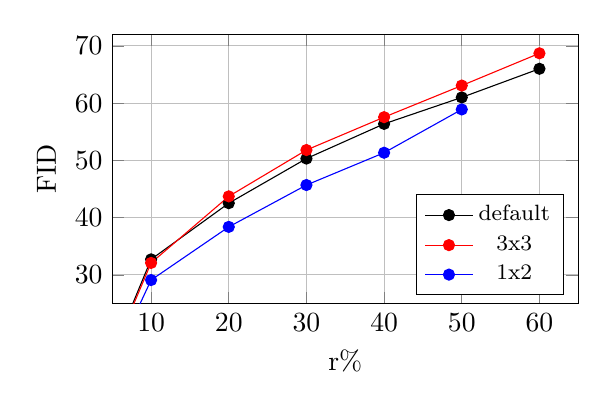
\begin{tikzpicture}
\begin{axis}[
    title={},
    height=5cm,
    width=7.5cm,
    xlabel={r\%},
    ylabel={FID},
    xmin=5, xmax=65,
    ymin=25, ymax=72,
    xtick={10,20,30,40,50,60},
    ytick={30,40,50,60,70},
    legend pos=south east,
    xmajorgrids=true,
    ymajorgrids=true,
    legend style={font=\footnotesize}
]

\addplot[
    color=black,
    mark=*
    ]
    coordinates {
    (0,0)(10,32.71)(20,42.52)(30,50.31)(40,56.37)(50,60.99)(60,65.99)
    };
    
\addplot[
    color=red,
    mark=*
    ]
    coordinates {
    (0,0)(10,32.09)(20,43.71)(30,51.80)(40,57.54)(50,63.06)(60,68.69)
    };

\addplot[
    color=blue,
    mark=*
    ]
    coordinates {
    (0,0)(10,29.10)(20,38.38)(30,45.69)(40,51.33)(50,58.89)
    };
    
\legend{default, 3x3, 1x2}
    
\end{axis}
\end{tikzpicture}
    % time values for run11, run14 and run15
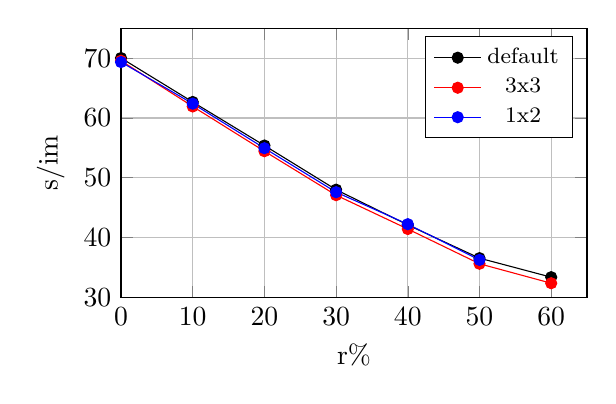
\begin{tikzpicture}
\begin{axis}[
    title={},
    height=5cm,
    width=7.5cm,
    xlabel={r\%},
    ylabel={s/im},
    xmin=0, xmax=65,
    ymin=30, ymax=75,
    xtick={0,10,20,30,40,50,60},
    ytick={30,40,50,60,70},
    legend pos=north east,
    xmajorgrids=true,
    ymajorgrids=true,
    legend style={font=\footnotesize}
]

\addplot[
    color=black,
    mark=*
    ]
    coordinates {
    (0,70.02)(10,62.67)(20,55.39)(30,48.01)(40,42.11)(50,36.56)(60,33.38)
    };
    
\addplot[
    color=red,
    mark=*
    ]
    coordinates {
    (0,69.56)(10,61.92)(20,54.44)(30,47.09)(40,41.43)(50,35.62)(60,32.37)
    };

\addplot[
    color=blue,
    mark=*
    ]
    coordinates {
    (0,69.34)(10,62.39)(20,54.94)(30,47.59)(40,42.24)(50,36.27)
    };
    
\legend{default, 3x3, 1x2}
    
\end{axis}
\end{tikzpicture}
\caption{FID and relative time compared to r=0\% for 3)}
\label{fig:exp_3}
\end{figure}\\
Resizing the batches only has minor effects on image generation speed, as all three configurations consistently remain within one second of each other, although the setup with $3 \times 3$ batch does consistently perform the best in that regard (see Tab.~\ref{table:exp_3}).\\
Image quality shows a noticeable improvement with smaller batch sizes. FID values for the ToMe setup using $3 \times 3$ batches slightly exceed the ones of the setup with $2 \times 2$ batches when \(r>10\%\), which in turn clearly exceed the ones of the version with $1 \times 2$ batches. (see Fig.~\ref{fig:exp_3}).
The gap closes towards \(r=50\%=r_{max}\), as every \textbf{src} token has to be merged when using $1 \times 2$ batches, regardless of how good of a match from \textbf{dst} is available.\\
It can still be concluded that using the $1 \times 2$ batches to create an equal number of \textbf{src} and \textbf{dst} tokens yields the best performance (even at a minor speed discount), especially when \(r\) is not close to \(0\%\) or \(r_{max}\), while the usage of larger batches with a smaller \(\textbf{dst\%}\) is not advisable.



%\newpage
\subsubsection*{4): Putting it all together}
Finally, we are comparing the most successful configurations from the past experiments. That means we are looking at \textbf{setup 1}: the ToMe default by Bolya and Hofmann (black), \textbf{setup 2}: our new default with token merging expanded to the cross-attn layer from \(1.2\) and \(1.4\) (red), and \textbf{setup 3}: the new default but with $1 \times 2$ batches for token partitioning from \(3.2\) (blue).\\
We expanded the image sets for the first two configurations to 1000 images per merge volume in \(1.4\), so we will do the same for the other one to enable examinations on a larger scale.
\begin{figure}[!htb]
    % FID values for run4, run16 (tbd)
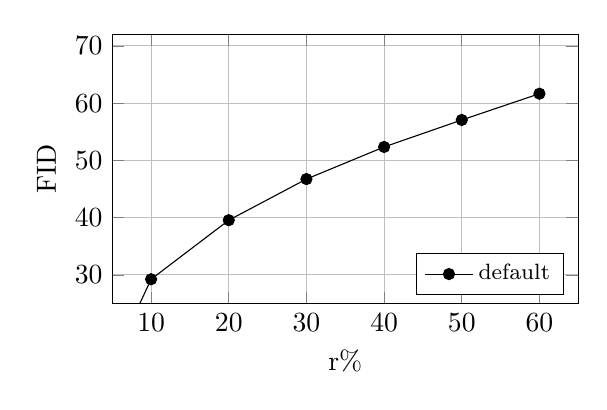
\begin{tikzpicture}
\begin{axis}[
    title={},
    height=5cm,
    width=7.5cm,
    xlabel={r\%},
    ylabel={FID},
    xmin=5, xmax=65,
    ymin=25, ymax=72,
    xtick={10,20,30,40,50,60},
    ytick={30,40,50,60,70},
    legend pos=south east,
    xmajorgrids=true,
    ymajorgrids=true,
    legend style={font=\footnotesize}
]

\addplot[
    color=black,
    mark=*
    ]
    coordinates {
    (0,0)(10,29.24)(20,39.55)(30,46.73)(40,52.34)(50,57.05)(60,61.64)
    };
    
\addplot[
    color=red,
    mark=*
    ]
    coordinates {
    
    };
    
\legend{default, 1x2}
    
\end{axis}
\end{tikzpicture}
    % time values for run2/10, run4/11, run15/16
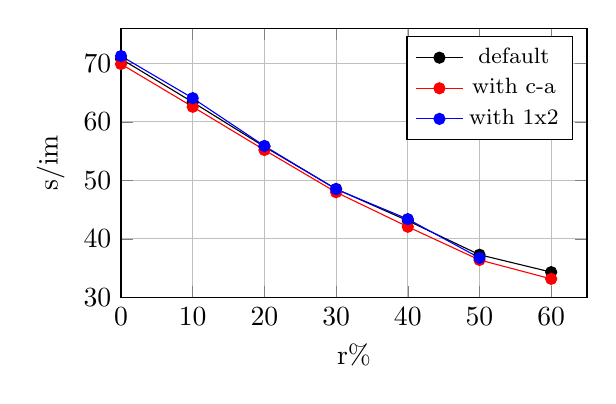
\begin{tikzpicture}
\begin{axis}[
    title={},
    height=5cm,
    width=7.5cm,
    xlabel={r\%},
    ylabel={s/im},
    xmin=0, xmax=65,
    ymin=30, ymax=76,
    xtick={0,10,20,30,40,50,60},
    ytick={30,40,50,60,70},
    legend pos=north east,
    xmajorgrids=true,
    ymajorgrids=true,
    legend style={font=\footnotesize}
]

\addplot[
    color=black,
    mark=*
    ]
    coordinates {
    (0,70.76)(10,63.36)(20,55.75)(30,48.53)(40,43.10)(50,37.29)(60,34.32)
    };
    
\addplot[
    color=red,
    mark=*
    ]
    coordinates {
    (0,69.88)(10,62.57)(20,55.19)(30,47.97)(40,42.07)(50,36.40)(60,33.16)
    };

\addplot[
    color=blue,
    mark=*
    ]
    coordinates {
    (0,71.25)(10,64.05)(20,55.88)(30,48.49)(40,43.38)(50,36.75)
    };
    
\legend{default, with c-a, with 1x2}
    
\end{axis}
\end{tikzpicture}
\caption{FID and relative time compared to r=0\% for 4)}
\label{fig:exp_4}
\end{figure}\\
Speed is very close across the board, with the speedup offered by every version always differing by less than 1.2\%. Within these thin margins, \textbf{Setup 2} consistently beat \textbf{Setup 1} when \(r>30\%\) and \textbf{Setup 3} was the quickest of the three most of the time (see Tab.~\ref{table:exp_4}).
Our discoveries regarding image quality are reinforced, with \textbf{setup 3} noticeably outperforming \textbf{setup 2}, which in turn performs slightly better than \textbf{setup 1} (see Fig.~\ref{fig:exp_4}).\\



%\newpage
\subsubsection*{Summary}
The experiments we conducted suggest that the best performance can be achieved by applying token merging in both the self-attn and cross-attn layer of the transformer. Depending on whether speed or image quality is the most important demand, $1 \times 2$ (best image quality) or $2 \times 2$ batches (highest speed) can be chosen for token partitioning, with $1 \times 2$ batches bringing particularly great improvements to image quality when \(r\leq40\%\).\\
Another important discovery is that token merging in the self-attn module is essential to unlocking speed improvements for image generation. On the other hand, using ToMe in the mlp layer seems to exclusively come at a disadvantage.\\
Moreover, it is important to create sufficiently large images when using ToMe in order to see the speed benefits. We showed that the time improvements with token merging noticeably decrease from >50\% for $768 \times 768$ images to only about 25\% for $512 \times 512$ images at \(r=60\%\) (see Tab.~\ref{table:exp_1_4},~\ref{table:exp_2}).\\
Additionally, it was shown that strongly skewing the \textbf{src}-\textbf{dst}-ratio away from an equal distribution has negative effects on image quality as well (see Tab.~\ref{table:exp_2}).
